\chapter{Detector de personas multi-escala}
En este apartado se describen la implementación de un detector de personas con uno de los modelos utilizados anteriormente. El proceso descrito en este apartado se puede encontrar en el fichero \textbf{multiscale.py}

\section{Implementación detector de personas}
Para implementar el detector de personas se ha implementado la clase \textit{PedestrianDetector}. Dicha clase utiliza el mejor modelo encontrado en validación de SVM con kernel lineal con HOG; se ha elegido este modelo por tener un buen rendimiento y su rápidez para cálcular las predicciones. Para poder cargar este modelo dentro de la clase se ha utilizado la función \textit{cv.ml.SVM\_load()} que permite cargar un modelo ya entrenado que haya sido entrenado anteriormente; para guardar el modelo hay que utilizar la función \textit{modelo\_svm.save()} indicando el nombre del fichero donde se guardará el modelo, este fichero debe ser \textit{.xml}. El modelo que se ha guardado es el modelo que devuelve la función \textit{crossValidation()}. \\

Dentro de la clase \textit{PedestrianDetector} hay varios métodos implementados que se utilizan para cuando el detector calcula si hay personas en la imagen. El primer método \textit{createPyramid()}, este tiene como argumento la imagen en la que se quiere detectar personas; lo único que hace este método es devolver un vector con la imagen a diferentes tamaños, estos son la imagen original, la imagen a la mitad de tamaño, a un cuarto de su tamaño, y la imagen a $1.5$ de su tamaño; y un vector con la escala de cada una de las imágenes para poder pasar transformar la posición de las ventanas detectadas en diferentes escalas a la escala original. El segundo método es \textit{computeWindows()} que tiene como argumentos un imagen y el desplazamiento de la ventana deseado; este método calcula el descriptor HOG desplazando la ventana por la imagen y devuelve una matriz con los resultados de cada ventana y la posición inicial de cada ventana calculada para después poder dibujar un rectángulo si dicha ventana es clasificada como contenedora de una persona. El tercer método es \textit{checkIfInRange()}, este método calcula si una ventana que contiene a una persona está en rango (esta cerca) de otra ventana elegida anteriormente, de esta forma se intenta evitar que haya más de una ventana por persona detectada. Por último, está el método \textit{compute2()}, esta función se le pasa la imagen para la cual queremos detectar personas; básicamente, esta función llama a las funciones descritas anteriormente y dibuja las ventanas elegidas finalmente y muestra los resultados por pantalla.

\section{Pruebas con imágenes}
En esta sección se mostrarán los resultados obtenidos para tres imágenes diferentes.

\begin{figure}[H]
	\centering
	\subfigure{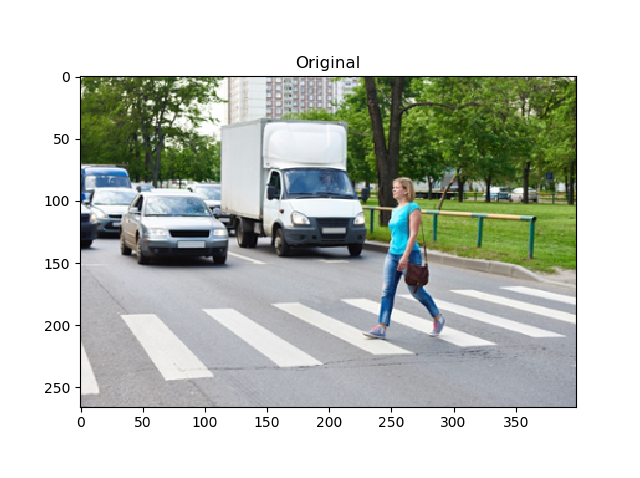
\includegraphics[width=80mm]{imagenes/prueba_1}}
	\subfigure{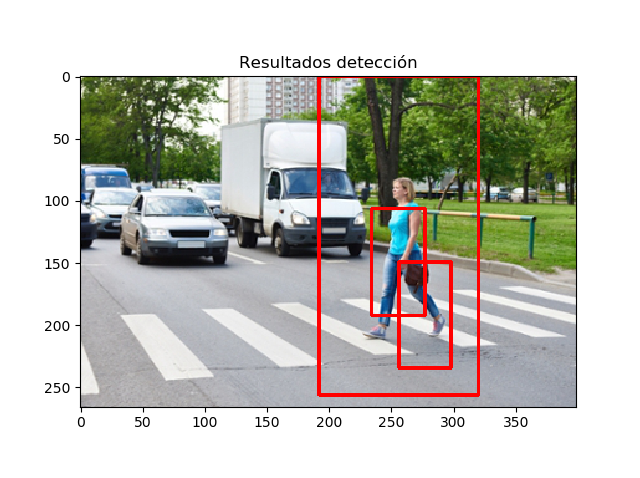
\includegraphics[width=80mm]{imagenes/resultado_1}}
	\caption{Prueba detección de personas 1}
	\label{fig:resultados1}
\end{figure}

\newpage

\begin{figure}[H]
	\centering
	\subfigure{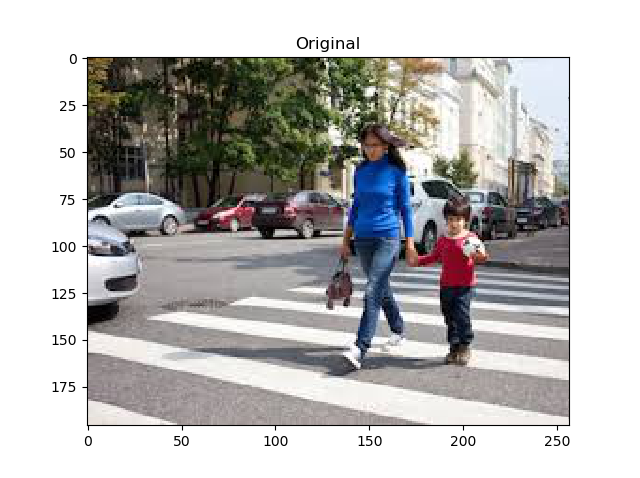
\includegraphics[width=80mm]{imagenes/prueba_2}}
	\subfigure{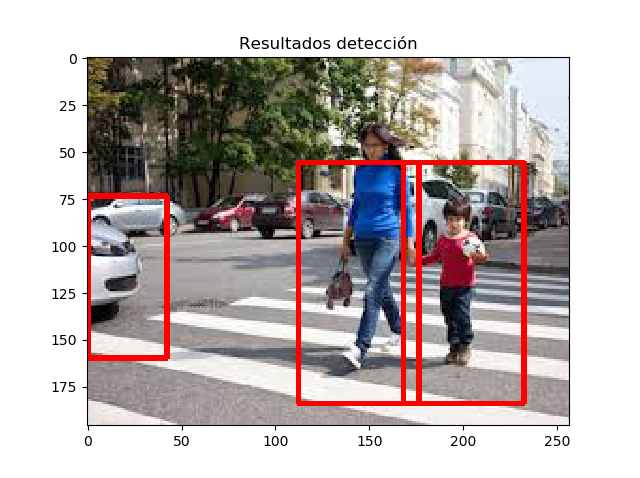
\includegraphics[width=80mm]{imagenes/resultado_2}}
	\caption{Prueba detección de personas 2}
	\label{fig:resultados2}
\end{figure}

\newpage

\begin{figure}[H]
	\centering
	\subfigure{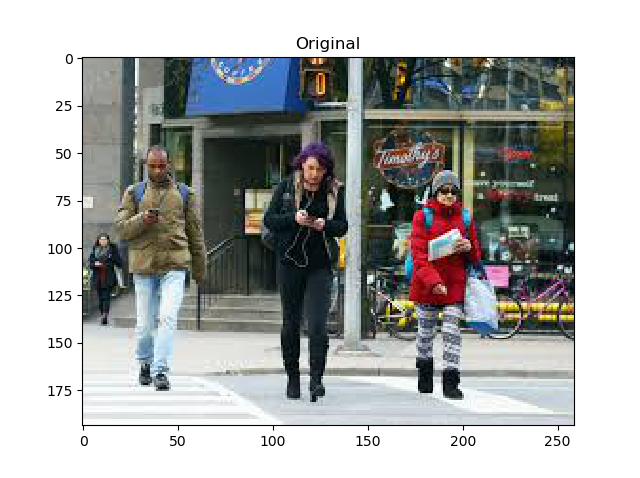
\includegraphics[width=80mm]{imagenes/prueba_3}}
	\subfigure{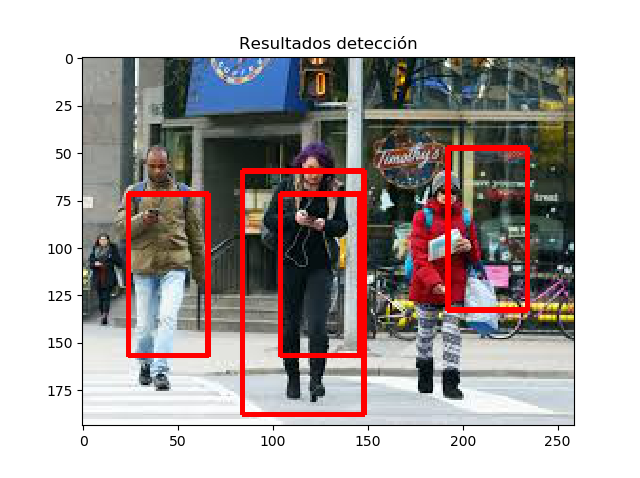
\includegraphics[width=80mm]{imagenes/resultado_3}}
	\caption{Prueba detección de personas 3}
	\label{fig:resultados3}
\end{figure}


